%! Author = ia
%! Date = 4/22/22

% Preamble
\documentclass[11pt]{article}

% Packages
\usepackage{amsmath}

% Document
\begin{document}

%% %%%%%%%%%%%%%%%%%%%%%%%%%%%%%%%%%%%%%%%%%%%%%%%%%%%%%%%%%%%%%%%%%%%%%%%%%%%%%%%%%%%%%%%%%%%%%%%%%%%%%%%%%%

	\section{\normalsize{Appendix: Comparing Models and Empirical Data}}

	In this section we compare the theoretical models defined above with empirical chain data
	for Ethereum and Ethereum Classic to both affirm the validity of the models as well
	as develop our understanding of observable network and chain behavior.

	\subsection{\normalsize{Orphan/Uncle Rate}}

%Orphans are blocks which are valid but do not eventually become canonical.
%Uncles are orphans which have been included in chain data via the \mghost protocol.
%As such, an uncle rate can be estimated by chaindata observation.

	The observable uncle rate should be expected to be at least, but not more than, predicted orphan rates.
	All orphans recorded as uncles on chain must be valid, but not all orphans must be recorded.\footnote{
		The recording of orphans as uncles is allowed but not mandated (or enforceable) by chain protocol.
		However, miners are rewarded for each uncle reference, and thus are incentivized to do so.
	}

	At the time of writing, Etherscan.io\footnote{\url{https://etherscan.io/uncles}}
	shows $1,256,671$ recorded uncles and a current canonical height of $14,610,325$ for Ethereum.

	\begin{equation}
		1256671 / 14610325 =  0.0860125
	\end{equation}

	We interpret this as representing an orphan rate of about 8.7\%.

	As noted earlier, the difference between the theoretical 6.8\% and observed 8.7\% is rationalizable by
	the difference between assumed and actual latency and block interval values.\footnote{
		Given observed uncle rates, we can use the model to estimate actual latency between miners.
		For example, the values $\lambda = 13.48$ and $t = 1.23$ yield a probability of $8.7\%$,
		suggesting actual miner-miner latency of around 1.23 seconds.
	}

	While it has been suggested that uncles represent a signal of near-simulaneous block emission events,
	not all uncles are losers of symmetric events.
	Uncles can be "born-losers," too. They are records of valid blocks which are not canonical.
	Under the current Ethereum and Ethereum Classic chain protocol,
	it is not expected that uncles are intentionally produced.\footnote{
		However, this has not always been the case.
		Uncle mining was, in fact, quite profitable at one time on Ethereum.
		EIP-100 modifies difficulty adjustment to prohibit an "issuance rate" from being
		"manipulated upward by manipulating the uncle rate."
		\url{https://github.com/ethereum/EIPs/blob/master/EIPS/eip-100.md#rationale=}.
	}

	\subsection{\normalsize{Canonical Emission Rate}}

	We examined recent and comparable data\footnote{
		Blocks 13 million through 14 million on both chains.
	} from the Etherum (ETH) and Ethereum Classic (ETC) blockchains
	to determine empirical estimates for incumbent-protocol emission rates.

	These data are charted as histograms\footnote{
		Source code for the analysis is included in the repository under \texttt{./empirical}.
	} in the following two figures.

	\begin{figure}[tph!]
		\centering
		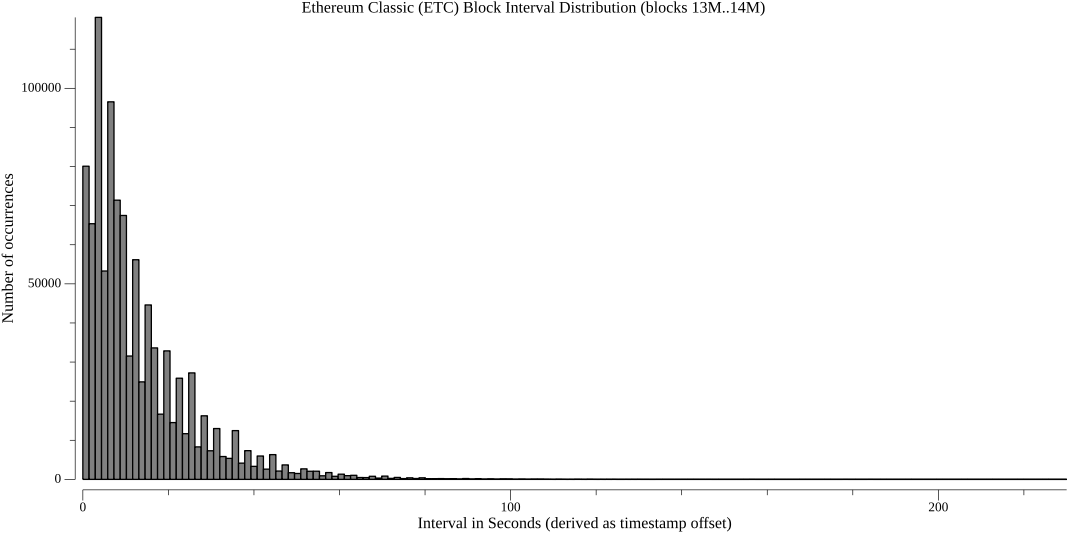
\includegraphics[width=1.0\textwidth]{vis_data_blockinterval_distribution_ETC.png}
		\caption{
			Exemplary block interval data for Ethereum Classic.\footnote{Source: \texttt{empirical/ETC}}
		}
	\end{figure}

	\begin{figure}[tph!]
		\centering
		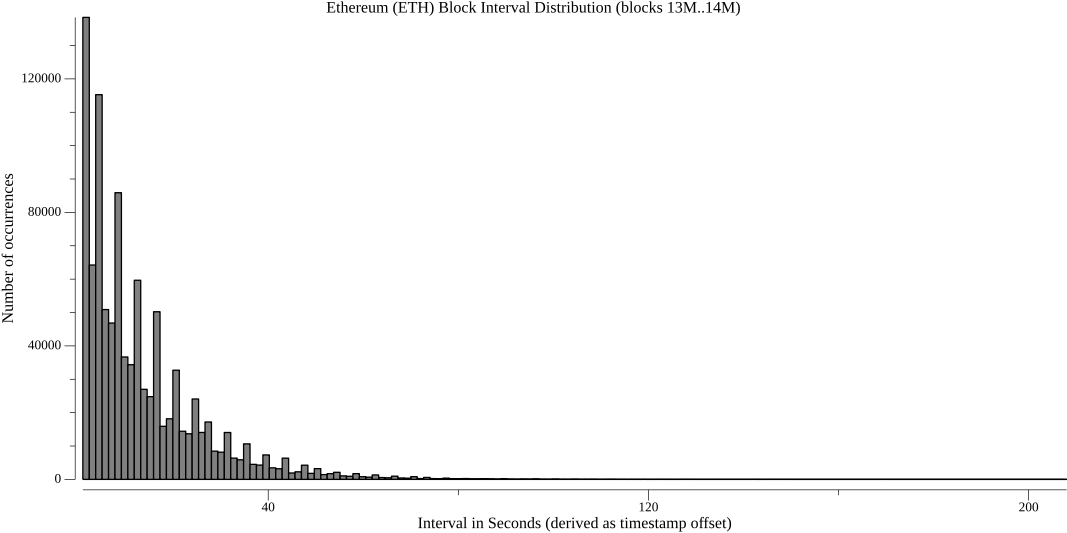
\includegraphics[width=1.0\textwidth]{vis_data_blockinterval_distribution_ETH.png}
		\caption{
			Exemplary block interval data for Ethereum.\footnote{Source: \texttt{empirical/ETH}}
		}
	\end{figure}

	\clearpage

	The mean block time for both networks is approximately 13.5 seconds for both chains.
	From this, for the sake of argument, we assume a general mean block interval as 14 seconds.

	Next, we use a computer program to simulate block intervals under the Poisson
	model.\footnote{\texttt{TestPoissonIntervals}}

	\begin{figure}[tph!]
		\label{vis_poisson_samples_events_86400}
		\centering
		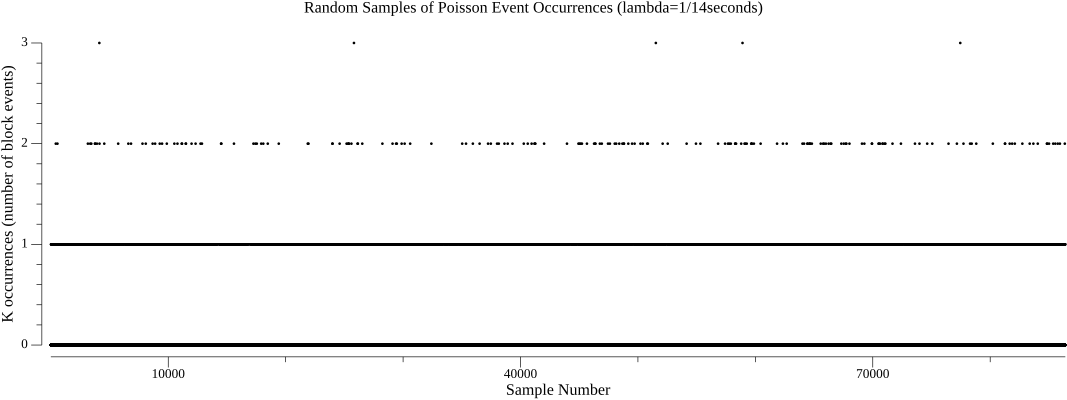
\includegraphics[width=1.0\textwidth]{go-block-step/out/vis_poisson_samples_events_86400.png}
		\caption{
			Procedurally generated event occurrence samples from a Poisson distribution
			with $\lambda = \frac{1}{14}$, sample size of 86400.
			We can interpret the data points at $y=2$ in Figure 20 and Figure 21 as
			representative of occurrences of forks having 2 candidate blocks.
			For $y=3$, the sample has 3 candidate blocks, etc.
		}
	\end{figure}

	\begin{figure}[tph!]
		\label{vis_poisson_samples_eventintervals_hist}
		\centering
		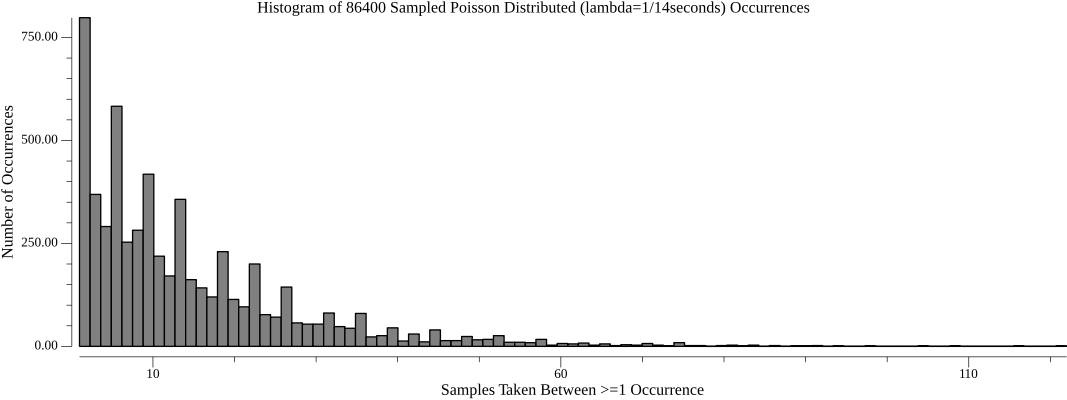
\includegraphics[width=1.0\textwidth]{go-block-step/out/vis_poisson_samples_eventintervals_hist.png}
		\caption{
			Procedurally generated intervals of samples where events $\geq 1$ from
			a Poisson distribution with $\lambda = \frac{1}{14}$.
		}
	\end{figure}

%The  represents derivative data from original sample values presented in
%the following plot, Figure 20.

%The same program is reused with a smaller sample size to produce a data set
%(shown in Figure 21) making the intervals between $r >= 1$ occurrences (for
%time interval 1 second) more observable:
%
%\begin{figure}[tph]
%    \centering
%    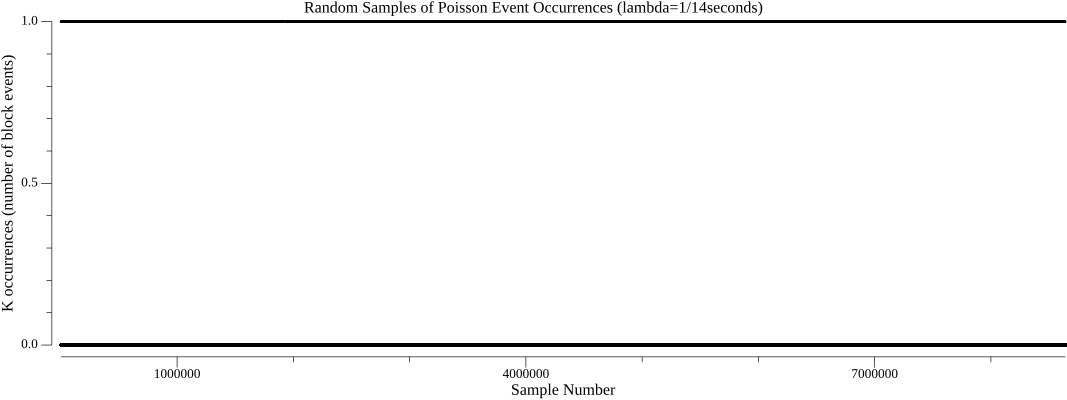
\includegraphics[width=1.0\textwidth]{go-block-step/out/vis_poisson_samples_events_8640000.png}
%    \caption{
%      Procedurally generated event interval samples from a Poisson distribution
%with $\lambda = \frac{1}{14}$, with a sample size of 8640000.
%    }
%\end{figure}


\end{document}